\PassOptionsToPackage{table}{xcolor}
\documentclass[12pt]{article}
\usepackage[utf8]{inputenc}
\usepackage[spanish]{babel}
\usepackage[margin=2.5cm]{geometry}
\usepackage{graphicx}
\usepackage{enumitem}
\usepackage{hyperref}
\hypersetup{
    colorlinks=true,
    linkcolor=black,
    urlcolor=blue,
    citecolor=black
}
\usepackage{eso-pic}
\usepackage{float}
\usepackage{transparent}
\usepackage{tikz}
\usepackage[nottoc]{tocbibind}
\usepackage{booktabs}
\usepackage[style=ieee, backend=bibtex]{biblatex}
\usepackage{csquotes}
\usepackage{amsmath,amssymb}
\usepackage{listings}
\usepackage{xcolor}
\usepackage[T1]{fontenc}
\usepackage{lmodern}
\usepackage{array}
\usepackage{longtable}
\usepackage{tabularx}
\usepackage[most]{tcolorbox}

\setcounter{secnumdepth}{4}
\setcounter{tocdepth}{4}

\usepackage{titlesec}

\titleformat{\paragraph}
{\normalfont\normalsize\bfseries}
{\theparagraph}
{1em}
{}

\titlespacing*{\paragraph}
{0pt}
{1.5ex plus 1ex minus .2ex}
{1ex}

\usetikzlibrary{arrows.meta,positioning}

\geometry{margin=2.5cm}
\setlength{\parindent}{0pt}
\setlength{\parskip}{0.8em}
\renewcommand{\arraystretch}{1.25}

\definecolor{verdeEncabezado}{HTML}{70AD47}
\definecolor{verdeClaro}{HTML}{E2F0D9}
\definecolor{amarilloEncabezado}{HTML}{FFC000}
\definecolor{amarilloClaro}{HTML}{FFF2CC}
\definecolor{codigoFondo}{HTML}{F7F7F7}

\lstdefinestyle{yamlStyle}{
    basicstyle=\ttfamily\small,
    numbers=left,
    numberstyle=\tiny\color{gray},
    stepnumber=1,
    numbersep=5pt,
    backgroundcolor=\color{gray!10},
    frame=single,
    breaklines=true,
    tabsize=2,
    showstringspaces=false,
    captionpos=b,
    keywordstyle=\color{blue}\bfseries,
    commentstyle=\color{green!50!black}\itshape,
    stringstyle=\color{red},
    morekeywords={
        openapi,info,title,version,description,servers,url,paths,get,post,put,delete,
        summary,tags,parameters,name,in,required,schema,type,responses,content,
        application/json,requestBody,components,schemas,items,properties,format,ref
    },
    sensitive=false
}

\lstdefinestyle{codigo}{
    backgroundcolor=\color{codigoFondo},
    basicstyle=\ttfamily\small,
    breaklines=true,
    breakatwhitespace=false,
    columns=fullflexible,
    keepspaces=true,
    showstringspaces=false,
    frame=single,
    rulecolor=\color{black!30},
    xleftmargin=1em,
    xrightmargin=1em
}


\lstdefinelanguage{Dockerfile}{
    keywords={FROM,RUN,COPY,WORKDIR,ENV,EXPOSE,CMD,AS},
    keywordstyle=\color{blue!70!black}\bfseries,
    basicstyle=\ttfamily\small,
    sensitive=true,
    comment=[l]{\#},
    commentstyle=\color{gray}\itshape,
    stringstyle=\color{red!60!black},
    morestring=[b]",
}

\lstdefinelanguage{yaml}{
    keywords={true,false,null,y,n},
    keywordstyle=\color{blue!70!black}\bfseries,
    basicstyle=\ttfamily\small,
    sensitive=false,
    comment=[l]{\#},
    commentstyle=\color{gray}\itshape,
    stringstyle=\color{red!60!black},
    morestring=[b]',
    morestring=[b]"
}

\addbibresource{referenciasPFC.bib}

\begin{document}

    \begin{titlepage}
        \AddToShipoutPicture* {
            \AtPageCenter{%
                \makebox(0,0){%
                    \begin{tikzpicture}[remember picture,overlay]
                    \IfFileExists{UteqLogo.png}{
                        \node[opacity=0.08] at (current page.center) {
                            
\includegraphics[width=9cm]{UteqLogo.png}
                        };
                    }{}
                    \end{tikzpicture}
                }%
            }
        }

        \centering
        {\scshape\large Universidad Técnica Estatal de Quevedo \par}
        {\scshape\large Facultad de Ciencias de la Computación \par}
        \vspace{0.8cm}

        {\large\textbf{PROYECTO FIN DE CURSO (PFC) --- ENTREGA 3}\par}
        \vspace{0.8cm}

        {\large\textbf{PROYECTO:}\par}
        \vspace{0.2cm}
        {\Large\textbf{TIENDATECH: IMPLEMENTACIÓN Y VALIDACIÓN DEL SISTEMA DISTRIBUIDO}\par}
        \vspace{0.7cm}

        {\large\textbf{MATERIA:}\par}
        \vspace{0.2cm}
        {\large APLICACIONES DISTRIBUIDAS \par}
        \vspace{0.7cm}

        {\large\textbf{DOCENTE:}\par}
        \vspace{0.2cm}
        {\large ING. GUERRERO ULLOA GLEISTON CICERON \par}
        \vspace{0.7cm}

        {\large\textbf{CURSO / PERÍODO ACADÉMICO:}\par}
        \vspace{0.2cm}
        {\large 7mo A --- PERÍODO ACADÉMICO 2026 \par}

        \vspace{1.0cm}

        {\large\textbf{INTEGRANTES:}\par}
        \vspace{0.25cm}
        {\normalsize
        Jhinson Stalyn Aucatoma Celorio \\
        Jeremy Ruperto Gaibor Rodriguez \\
        Andy Paul Sanchez Pilaloa \\
        José Alejandro Lozano Morales \par}
        \vspace{0.7cm}

        {\large\textbf{FECHA DE ENTREGA:}\par}
        \vspace{0.2cm}
        {\large 28 DE JULIO DE 2026 \par}
    \end{titlepage}

    \tableofcontents
    \newpage


    \section*{Resumen}
    \addcontentsline{toc}{section}{Resumen} % Para que aparezca en el índice sin numerar

    El proyecto \textbf{TiendaTech} implementa una plataforma de comercio electrónico especializada en componentes de hardware mediante una arquitectura distribuida. En esta tercera entrega se validó un despliegue compuesto por un frontend que centraliza el acceso y seis microservicios responsables de usuarios, productos, inventario, pedidos, órdenes a proveedores y ventas. Los siete componentes fueron contenerizados con Docker Compose y se conectaron a una base PostgreSQL compartida denominada \texttt{TiendaTechV19}. La validación funcional comprobó el flujo entre carrito, creación de orden, generación de factura y reducción automática del inventario. Se ejecutaron diez casos funcionales, todos satisfactorios, y 210 solicitudes secuenciales de lectura distribuidas en siete endpoints. La tasa de éxito fue del 100\,\% y el mayor percentil 95 observado fue de 51,94~ms, inferior al umbral de 500~ms definido para esta etapa. Los resultados confirman la integración básica del sistema distribuido y permiten identificar como trabajo posterior la ampliación de pruebas concurrentes, el aislamiento de datos y la implementación de capacidades aún no incorporadas.

    \vspace{1cm}

    \textbf{Palabras clave:} Microservicios, Comercio Electrónico, Sistemas Distribuidos, API REST, Docker, PostgreSQL.

    \newpage

    \section*{Abstract}
    \addcontentsline{toc}{section}{Abstract}

    TiendaTech implements an e-commerce platform for computer hardware components through a distributed architecture. This third deliverable validates a deployment composed of a frontend that centralizes access and six microservices responsible for users, products, inventory, orders, supplier orders, and sales. All seven components were containerized with Docker Compose and connected to a shared PostgreSQL database named \texttt{TiendaTechV19}. Functional validation covered the complete flow from the shopping cart to order creation, invoice generation, and automatic inventory reduction. Ten functional test cases were executed successfully, together with 210 sequential read requests distributed across seven endpoints. The observed success rate was 100\%, while the highest 95th percentile response time was 51.94~ms, below the 500~ms threshold defined for this stage. These results confirm the basic integration of the distributed system and identify concurrent testing, data isolation, and pending capabilities as future work.

    \vspace{1cm}

    \textbf{Keywords:} Microservices, Electronic Commerce, Distributed Systems, REST API, Docker, PostgreSQL.




    \section{Introducción}

    \subsection{Contexto y Problema Cuantificado}
    En la última década, el comercio electrónico en el Ecuador ha experimentado un crecimiento exponencial. Según datos oficiales de la Cámara Ecuatoriana de Comercio Electrónico (CECE), las transacciones digitales en el país han alcanzado una facturación anual que supera los 4,000 millones de dólares, donde la categoría de bienes tecnológicos y hardware informático se posiciona de forma consistente entre los tres sectores con mayor volumen de transacciones y demanda de mercado. Dentro de este ecosistema macroeconómico digital, el aprovisionamiento de computación personalizada de alto rendimiento exige plataformas comerciales que superen las capacidades de los catálogos estáticos tradicionales.

    El despliegue de plataformas nacionales complejas orientadas al comercio especializado requiere de la evolución de las arquitecturas de software tradicionales hacia sistemas distribuidos capaces de procesar información heterogénea en tiempo real \cite{vinayababu2025revolutionizing}. En este escenario nace \textbf{TiendaTech}, una plataforma centralizada de cobertura nacional diseñada no solo para capturar una cuota del flujo comercial cuantificado del hardware en el país, sino para automatizar la asistencia técnica mediante sistemas de software interactivos.

    \subsection{Definición del Problema y Brecha de Requerimientos Formales}
    El proceso de selección e integración de componentes para el armado de un computador representa un desafío crítico debido a la alta asimetría de información y a las estrictas dependencias de compatibilidad física, eléctrica y lógica entre las piezas. Un usuario se enfrenta al riesgo constante de adquirir componentes que presentan colisiones tecnológicas insalvables (como la disparidad de zócalos entre procesador y placa madre). En el contexto del e-commerce ecuatoriano actual, la mayoría de los sistemas operan bajo esquemas monolíticos que aíslan el inventario de las especificaciones de ingeniería del producto.

    Aquí se identifica una evidente \textbf{brecha de requerimientos formales (Brecha RQ)}: las plataformas comerciales vigentes cumplen con requerimientos transaccionales básicos (gestión de carrito, pasarela de pagos), pero carecen de requerimientos lógicos y formales de validación cruzada en tiempo real. Al no existir especificaciones formales automatizadas que validen las restricciones tecnológicas de los productos antes de la compra, el error del consumidor se detecta únicamente tras la entrega física, lo que desencadena ciclos ineficientes de devoluciones y pérdidas económicas para la empresa, evidenciando un vacío técnico que los sistemas monolíticos convencionales no pueden resolver.

    \subsection{Justificación de la Solución y Contribución Delimitada}
    Para mitigar la brecha identificada, \textbf{TiendaTech} se concibe bajo el paradigma de un sistema distribuido fundamentado en una arquitectura de microservicios. La implementación vigente separa usuarios, productos, inventario, pedidos, órdenes a proveedores y ventas, y utiliza un frontend con funciones de enrutamiento como punto de entrada. Esta separación permite validar el núcleo transaccional de comercio electrónico y constituye la base para incorporar posteriormente capacidades especializadas. Entre ellas se proyectan un motor de compatibilidad basado en restricciones \cite{velten2025solutions} y un asistente inteligente apoyado en Modelos de Lenguaje Grandes y arquitecturas RAG \cite{munson2025review}; ambos se mantienen fuera del alcance implementado y verificado en esta entrega.

    La \textbf{contribución delimitada} de la Entrega 3 comprende el despliegue contenerizado del frontend y seis microservicios, la comunicación REST entre los dominios principales y la validación del flujo carrito--orden--factura--inventario. Todos los servicios utilizan actualmente una base PostgreSQL compartida. Por tanto, el proyecto no declara todavía aislamiento de persistencia, alta disponibilidad productiva, motor de compatibilidad ni asistente inteligente; estas capacidades forman parte de la evolución propuesta.

    \section{Antecedentes arquitectónicos heredados de las Entregas 1 y 2}

    Con el objetivo de representar la estructura general del ecosistema distribuido de \textbf{TiendaTech}, se emplea el modelo arquitectónico C4, el cual permite describir sistemas de software complejos mediante diferentes niveles de abstracción.

    \subsection{Diagrama C4-L1: Contexto del Sistema}

    El diagrama C4 de nivel 1 permite visualizar la interacción global entre los usuarios externos y la plataforma distribuida \textbf{TiendaTech}. En este nivel se identifican los actores principales, así como los servicios externos en el flujo general de operación del sistema.

    \begin{figure}[H]
        \centering
        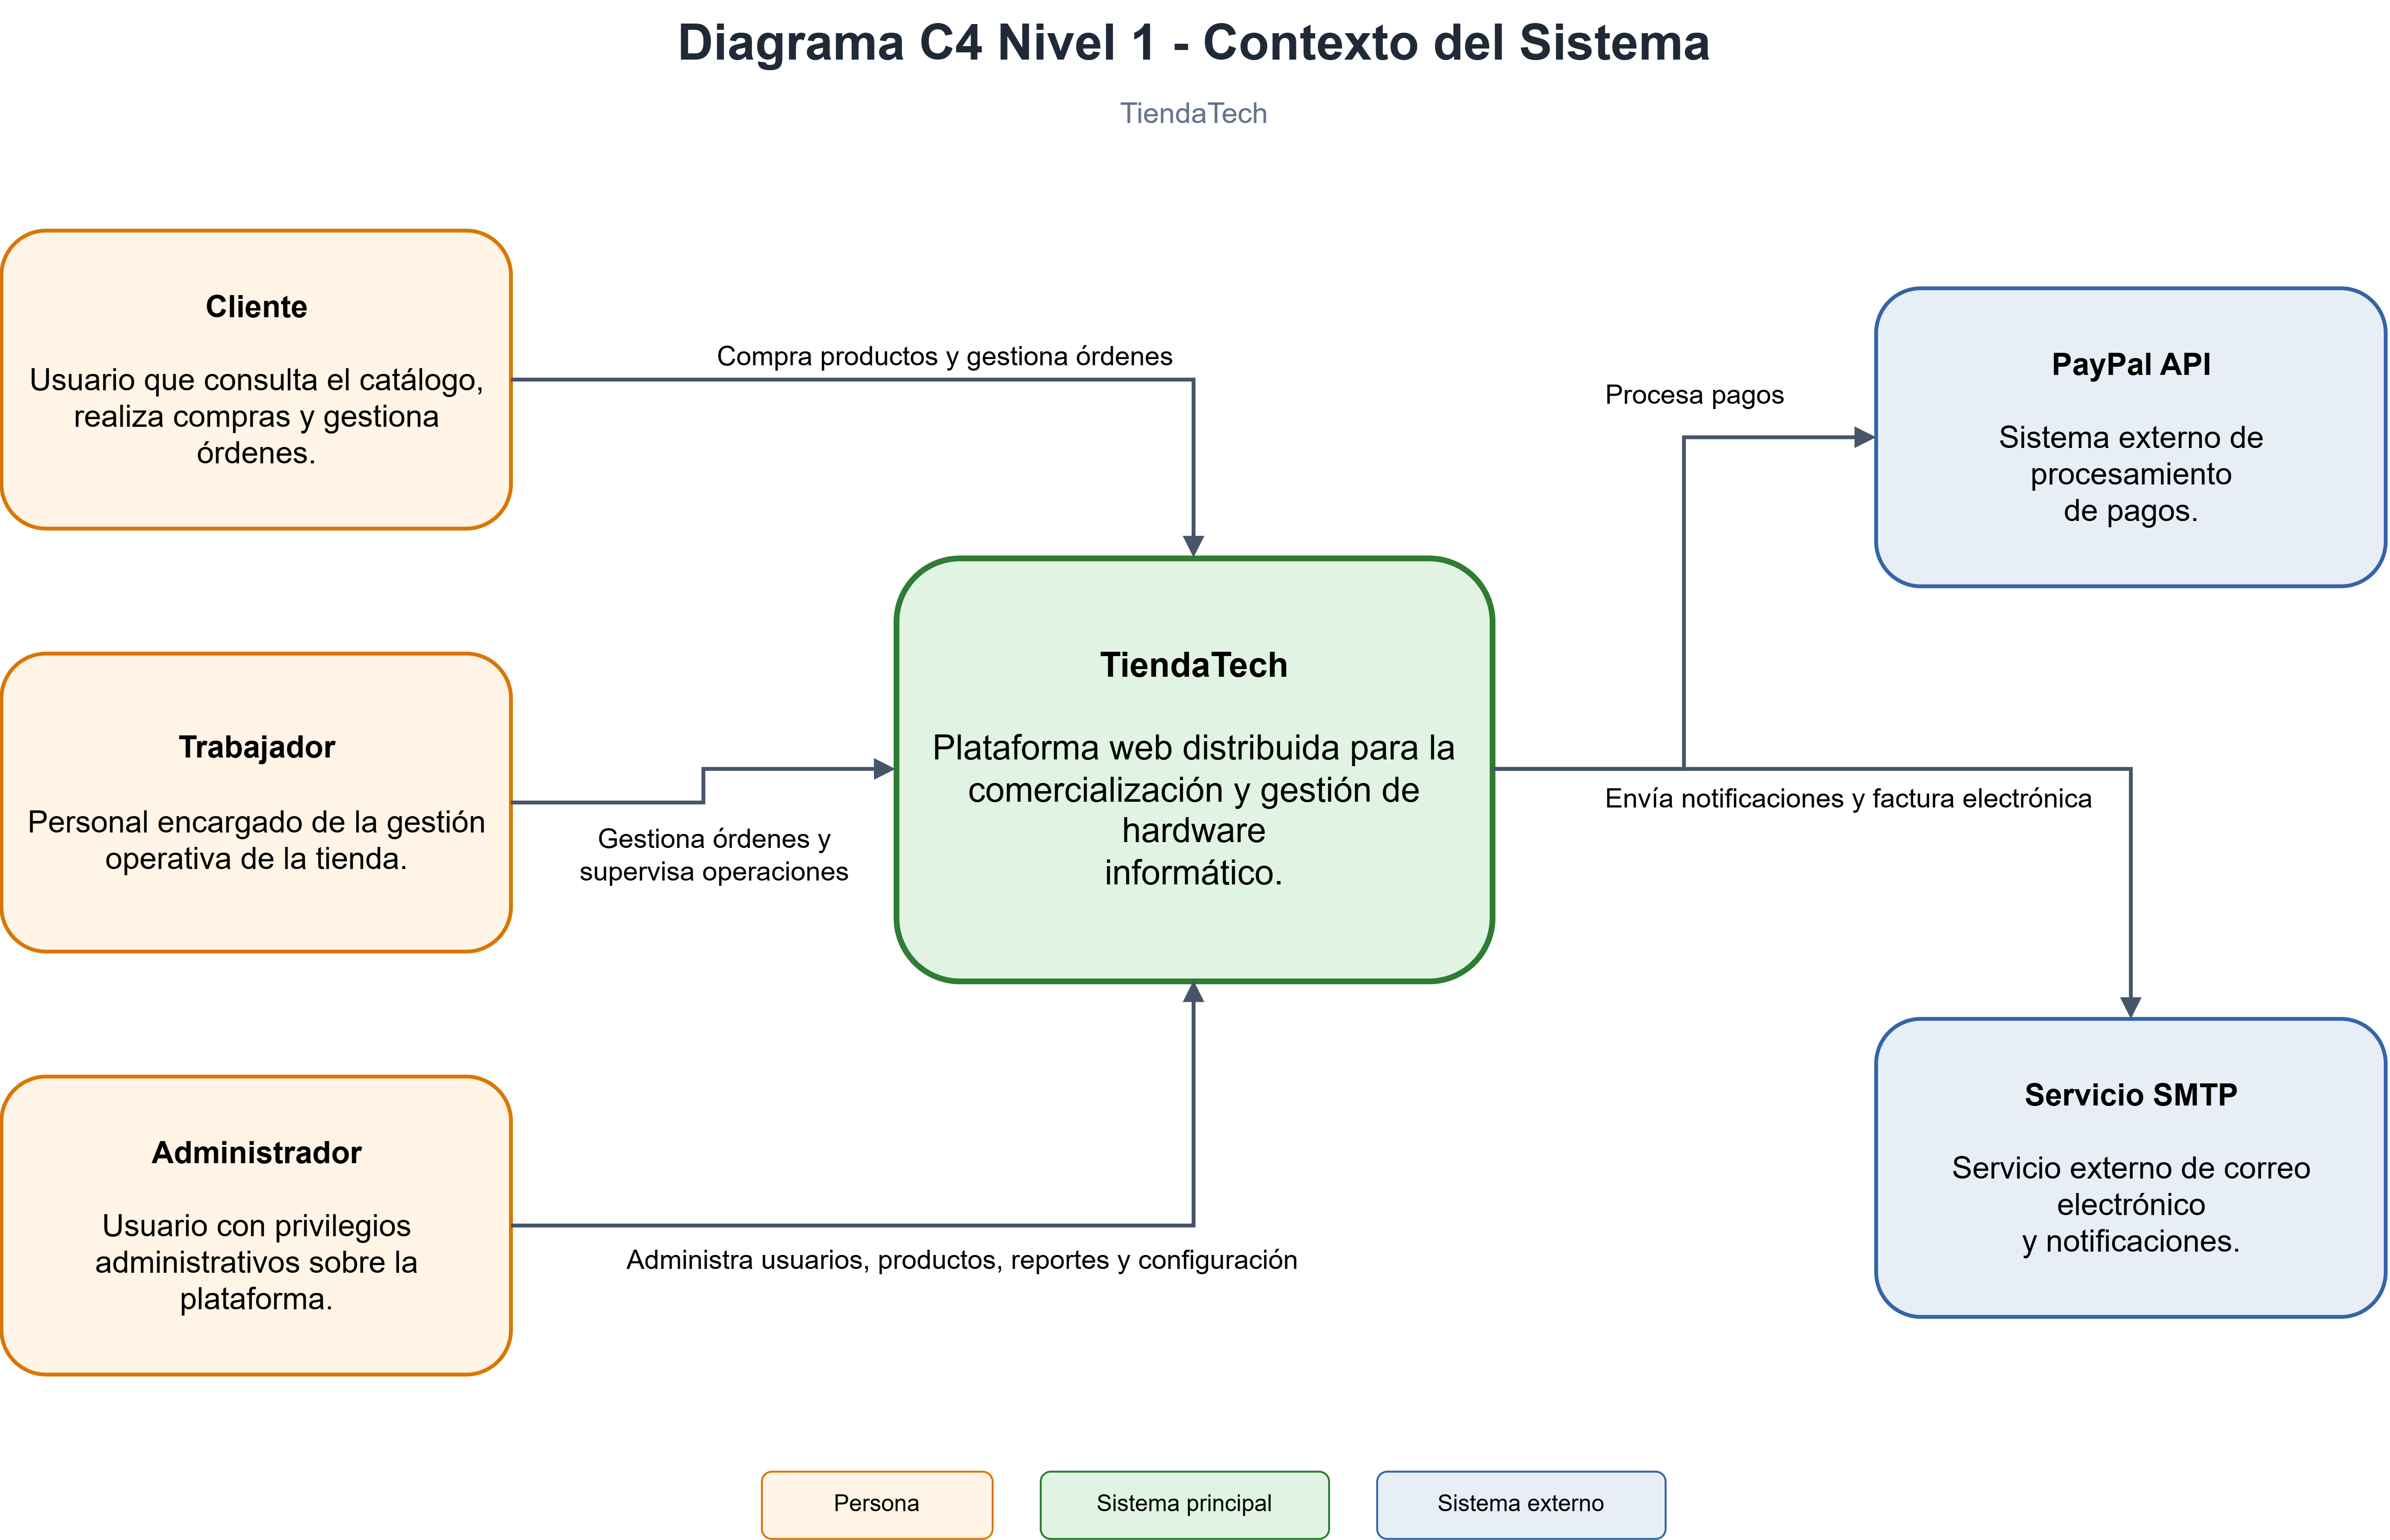
\includegraphics[width=\textwidth]{../diagrams/tiendatech-c4-l1.drawio.png}
        \caption{Diagrama C4-L1 del sistema distribuido TiendaTech.}
        \label{fig:c4l1}
    \end{figure}

    \subsection{Diagrama C4-L2: Diagrama de Contenedores}

    El diagrama C4 de nivel 2 representa la arquitectura efectivamente desplegada: un
    frontend basado en Spring Cloud Gateway y seis servicios Spring Boot. El frontend
    publica el puerto 8080 y enruta las solicitudes hacia Productos (8081), Inventario
    (8082), Pedidos (8083), Órdenes y proveedores (8084), Usuarios (8085) y Ventas
    (8086). Los servicios acceden actualmente a la base compartida
    \texttt{TiendaTechV19}.

    \begin{figure}[H]
        \centering
        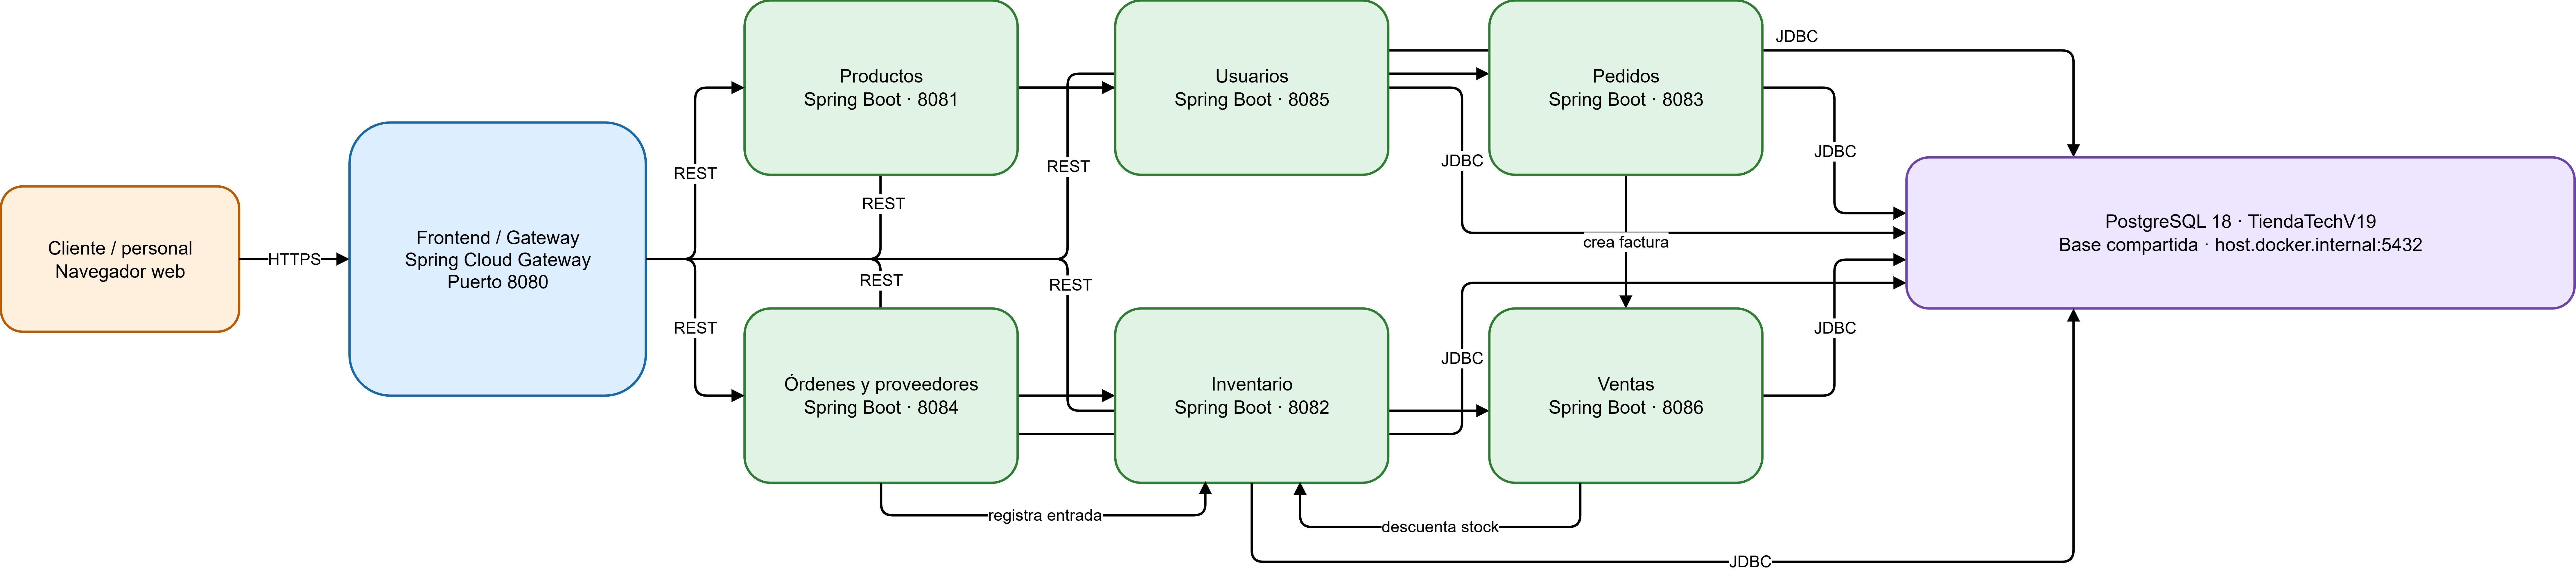
\includegraphics[width=\textwidth]{../diagrams/tiendatech-c4-l2.drawio.png}
        \caption{Diagrama C4-L2 de la arquitectura distribuida TiendaTech.}
        \label{fig:c4l2}
    \end{figure}

    \subsection{Diagrama C4-L3: Diagrama de Componentes}

    El nivel 3 se delimita al flujo de compra comprobado en esta entrega. El servicio de
    Pedidos coordina el carrito y el checkout, consulta Productos y Usuarios y solicita a
    Ventas la creación de la factura. Ventas registra posteriormente la salida mediante la
    interfaz REST de Inventario. El diagrama no incluye módulos de compatibilidad, pagos o
    notificaciones porque no forman parte del despliegue implementado y validado.

    \begin{figure}[H]
        \centering
        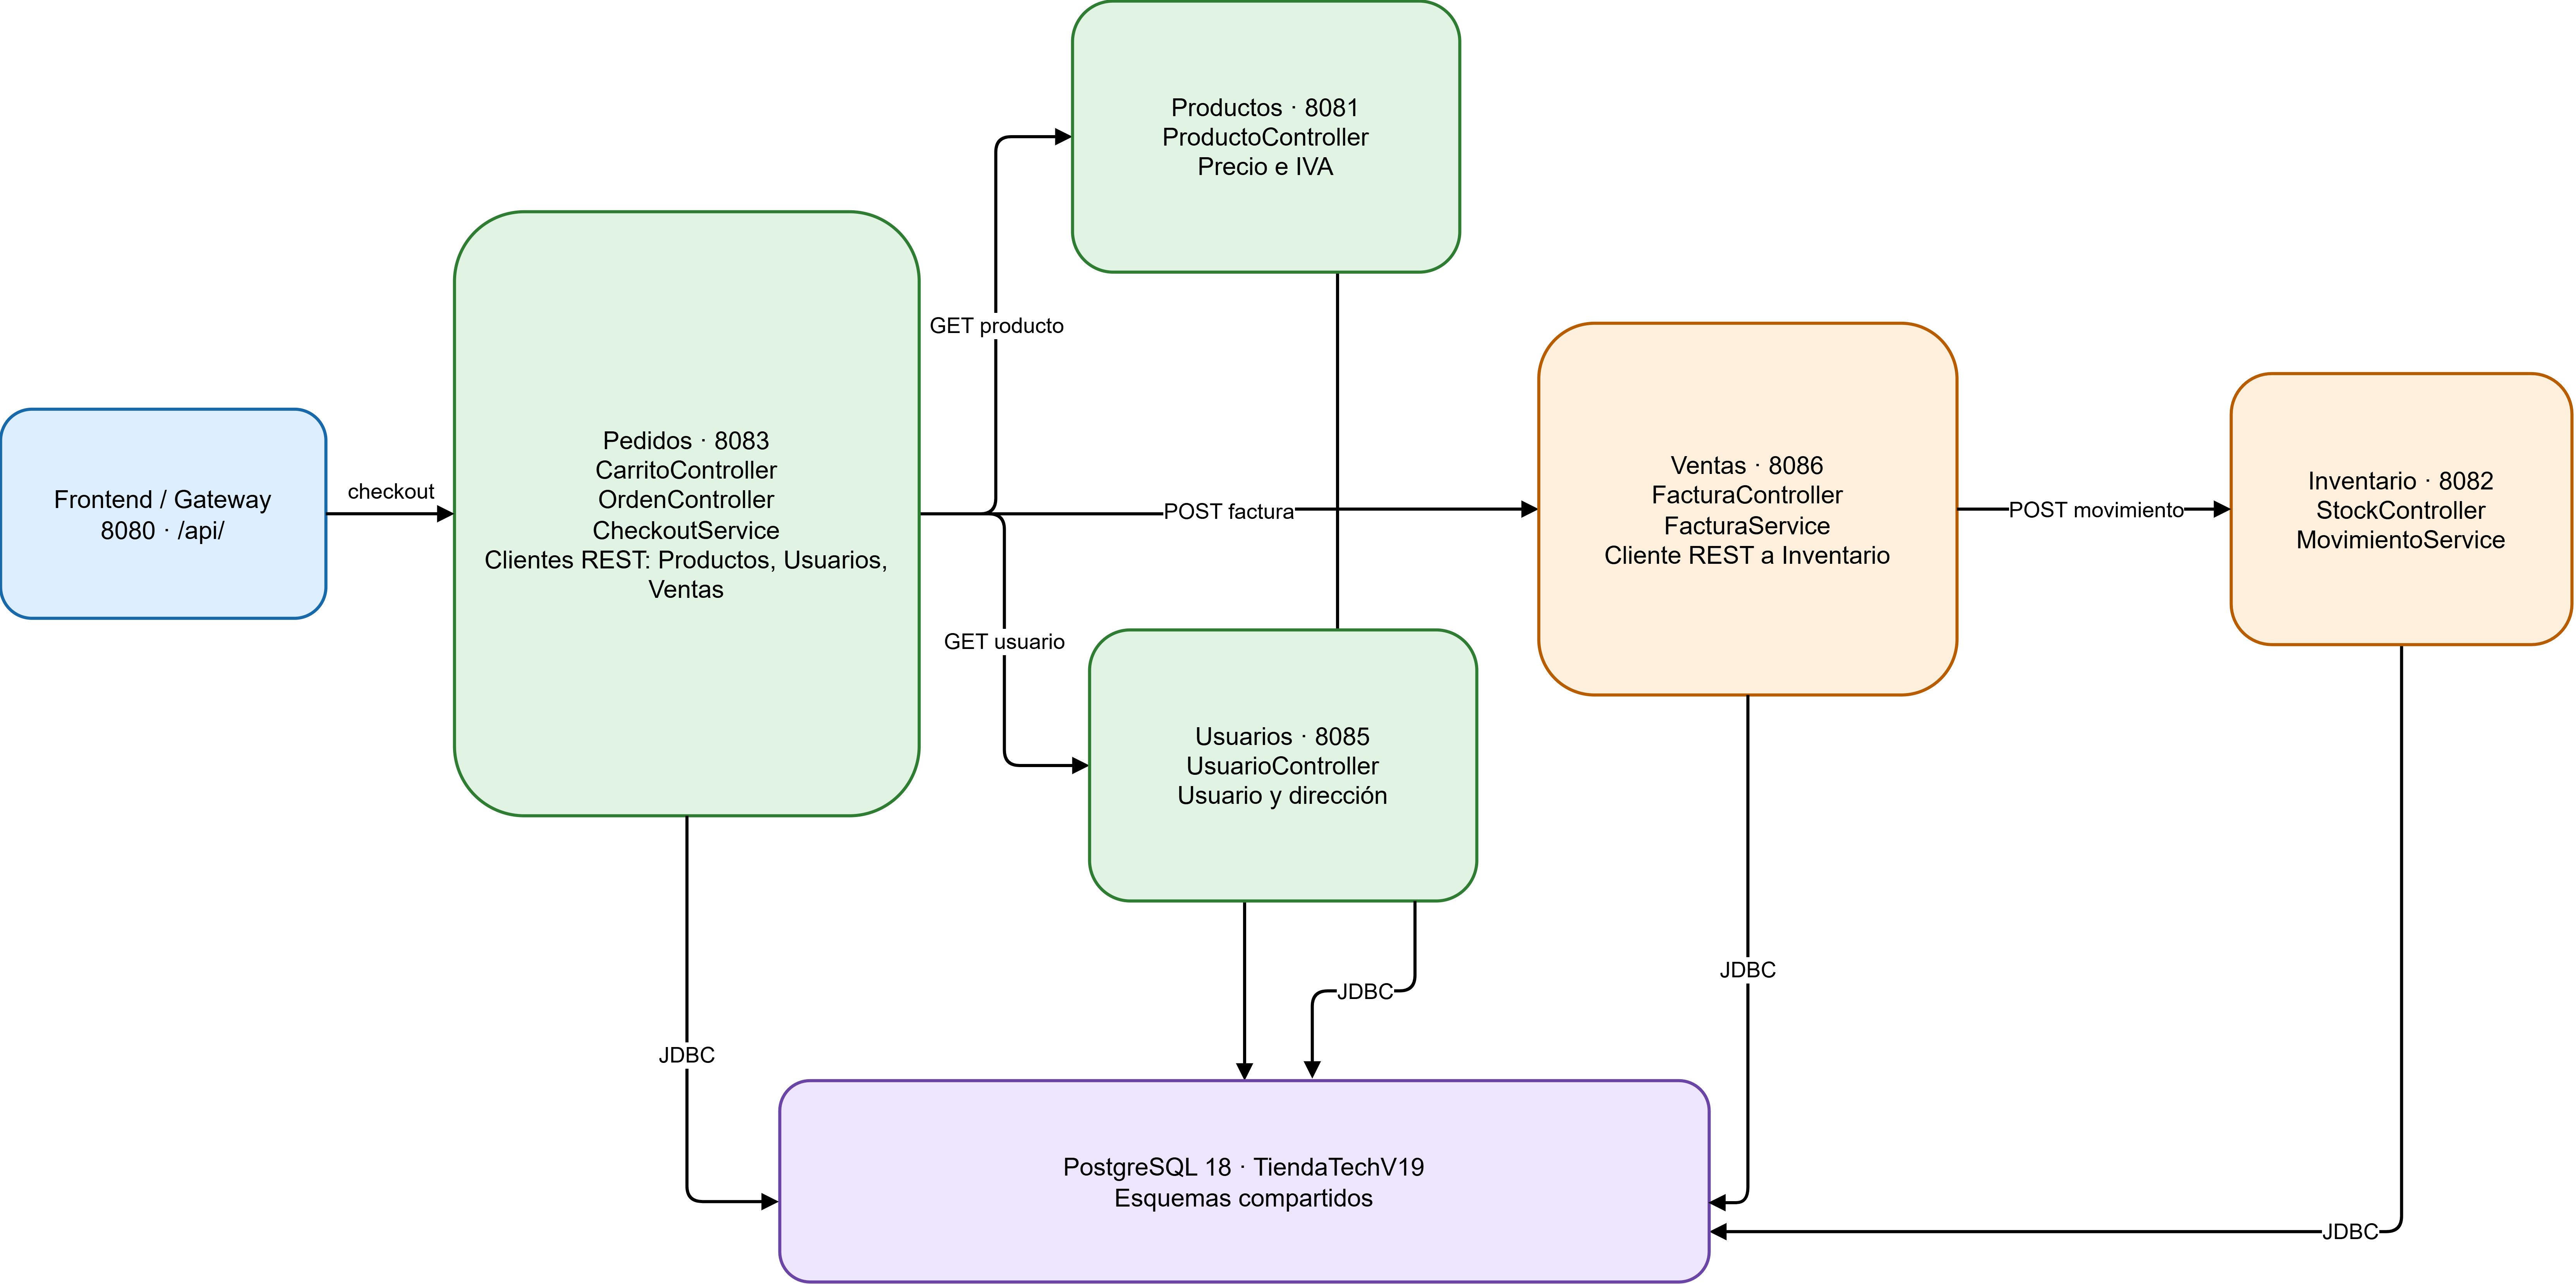
\includegraphics[width=\textwidth]{../diagrams/tiendatech-c4-l3-checkout.drawio.png}
        \caption{Diagrama C4-L3 de los componentes que participan en el checkout.}
        \label{fig:c4-l3-tiendatech}
    \end{figure}

    \subsection{Interfaces REST implementadas}

    La Entrega 2 planteó documentar contratos OpenAPI independientes. Sin embargo, los archivos YAML mencionados en aquella versión no se encuentran en el repositorio actual. Para mantener la trazabilidad entre el informe y la implementación, esta entrega documenta únicamente las interfaces REST verificadas directamente en los controladores y en las pruebas de integración. La formalización completa en OpenAPI permanece como deuda técnica.

    \begin{table}[H]
        \centering
        \caption{Interfaces REST principales verificadas en la Entrega 3}
        \label{tab:interfaces-rest-e3}
        \small
        \begin{tabularx}{\textwidth}{p{3.2cm} p{2cm} X}
\toprule
\textbf{Servicio} & \textbf{Método} & \textbf{Ruta y propósito} \\
\midrule
Productos & GET & \path{/api/productos/\{id\}}: consulta precio, IVA y datos del producto. \\
Inventario & GET & \path{/api/stock/\{productoId\}}: consulta el stock actual. \\
Inventario & POST & \path{/api/sp/movimiento-inventario}: registra entradas o salidas. \\
Pedidos & GET & \path{/api/carrito/\{usuarioId\}}: obtiene el carrito activo. \\
Pedidos & POST & \path{/api/ordenes/checkout}: crea la orden e inicia la facturación. \\
Usuarios & GET & \path{/api/usuarios/\{id\}}: consulta los datos mínimos del usuario. \\
Usuarios & GET & \path{/api/usuarios/\{id\}/direcciones}: valida direcciones habilitadas. \\
Ventas & POST & \path{/api/facturas}: genera una factura desde una orden. \\
Ventas & GET & \path{/api/facturas/\{id\}}: consulta el encabezado de factura. \\
Proveedores & GET & \path{/api/proveedores}: lista proveedores registrados. \\
\bottomrule
        \end{tabularx}
    \end{table}


    \subsection{Estrategia de contenerización del sistema distribuido}

    \paragraph{Tecnología utilizada}

    \begin{table}[htbp]
        \centering
        \caption{Herramientas utilizadas en el entorno de despliegue.}
        \label{tab:herramientas-despliegue}
        \small
        \begin{tabularx}{\textwidth}{>{\bfseries}l l X}
\toprule
Herramienta & Versión & Propósito \\
\midrule
Docker & 24+ & Contenerización de cada microservicio. \\
Docker Compose & V2 & Orquestación de todos los contenedores. \\
PostgreSQL & 18 & Motor de base de datos compartido en el host. \\
Eclipse Temurin JRE & 17 & Entorno de ejecución. \\
Maven & 3.9.9 & Compilación en etapa de \textit{build}. \\
\bottomrule
        \end{tabularx}
    \end{table}

    \paragraph{Estrategia de Bases de Datos}

    En el despliegue validado, todos los servicios utilizan la base PostgreSQL compartida
    \texttt{TiendaTechV19}, disponible en el host por el puerto 5432. El acceso desde los
    contenedores se realiza mediante \path{host.docker.internal}. El aislamiento de datos
    por servicio permanece como trabajo posterior.

    \begin{table}[htbp]
        \centering
        \caption{Asignación de contenedores de base de datos por microservicio.}
        \label{tab:contenedores-bd}
        \small
        \begin{tabularx}{\textwidth}{>{\bfseries}l X l}
\toprule
Microservicio & Contenedor BD & Puerto externo \\
\midrule
Usuarios y Seguridad & \texttt{tiendatech\_db\_usuarios} & 5433 \\
Productos & \texttt{tiendatech\_db\_productos} & 5434 \\
Inventario & \texttt{tiendatech\_db\_inventario} & 5435 \\
Pedidos & \texttt{tiendatech\_db\_pedidos} & 5436 \\
Ventas & \texttt{tiendatech\_db\_ventas} & 5437 \\
Órdenes y Proveedores & \texttt{tiendatech\_db\_ordenes} & 5438 \\
\bottomrule
        \end{tabularx}
    \end{table}

    Los datos se persisten mediante volúmenes Docker, lo que asegura que no se pierdan al reiniciar los contenedores.

    \paragraph{Comunicación entre microservicios}

    Todos los contenedores se conectan dentro de una red interna llamada \texttt{tiendatech\_net} de tipo \textbf{bridge}. Dentro de esta red, cada servicio se referencia por el \textbf{nombre de su contenedor} en lugar de una IP:

    \begin{tcolorbox}[colback=amarilloClaro,colframe=black,title=Ejemplos de comunicación interna]
        \begin{itemize}[leftmargin=1.5em]
    \item \texttt{pedidos-service $\rightarrow$ http://inventario-service:8083/api/inventario/...}
    \item \texttt{ventas-service $\rightarrow$ http://pedidos-service:8084/api/pedidos/...}
        \end{itemize}
    \end{tcolorbox}

    Esto hace que la comunicación sea independiente de la IP del host.

    \paragraph{Variables de entorno}

    La configuración sensible, como credenciales, URLs de servicios y claves, se inyecta mediante variables de entorno en el archivo \texttt{docker-compose.yml}, evitando hardcodear datos en el código fuente.

    \textbf{Ejemplo para el microservicio de Ventas:}

    \begin{lstlisting}[style=codigo]
environment:
  SPRING_DATASOURCE_URL: jdbc:postgresql://db_ventas:5432/db_ventas
  PEDIDOS_SERVICE_URL: http://pedidos-service:8084
  PAYPAL_CLIENT_ID: ${PAYPAL_CLIENT_ID}
  PAYPAL_CLIENT_SECRET: ${PAYPAL_CLIENT_SECRET}
    \end{lstlisting}

    \paragraph{Orden de arranque -- \texttt{depends\_on}}

    Se define el orden de inicio mediante \texttt{depends\_on} para evitar que un microservicio intente conectarse a su base de datos o a otro servicio antes de que estén disponibles:

    \begin{center}
        \begin{tikzpicture}[
            node distance=1.2cm and 1.8cm,
            servicio/.style={draw, rounded corners, minimum width=3.4cm, minimum height=0.8cm, fill=verdeClaro},
            bd/.style={draw, rounded corners, minimum width=3.4cm, minimum height=0.8cm, fill=amarilloClaro},
            flecha/.style={-Latex, thick, red!70!black}
        ]
\node[bd] (dbu) {db\_usuarios};
\node[servicio, right=of dbu] (usuarios) {usuario-service};
\node[bd, below=of dbu] (dbp) {db\_productos};
\node[servicio, right=of dbp] (productos) {productos-service};
\node[bd, below=of dbp] (dbi) {db\_inventario};
\node[servicio, right=of dbi] (inventario) {inventario-service};
\node[servicio, right=2.4cm of productos] (pedidos) {pedidos-service};

\draw[flecha] (dbu) -- (usuarios);
\draw[flecha] (dbp) -- (productos);
\draw[flecha] (dbi) -- (inventario);
\draw[flecha] (usuarios) -- (pedidos);
\draw[flecha] (productos) -- (pedidos);
\draw[flecha] (inventario) -- (pedidos);
        \end{tikzpicture}
    \end{center}

    \paragraph{Puertos expuestos}

    \begin{table}[htbp]
        \centering
        \caption{Puertos expuestos por los contenedores del sistema.}
        \label{tab:puertos-expuestos}
        \small
        \begin{tabularx}{\textwidth}{>{\bfseries}l l l}
\toprule
Contenedor & Puerto interno & Puerto externo \\
\midrule
\texttt{frontend} & 8080 & 8080 \\
\texttt{productos} & 8081 & 8081 \\
\texttt{inventario} & 8082 & 8082 \\
\texttt{pedidos} & 8083 & 8083 \\
\texttt{ordenes-proveedores} & 8084 & 8084 \\
\texttt{usuarios} & 8085 & 8085 \\
\texttt{ventas} & 8086 & 8086 \\
\bottomrule
        \end{tabularx}
    \end{table}

    \begin{figure}[H]
        \centering
        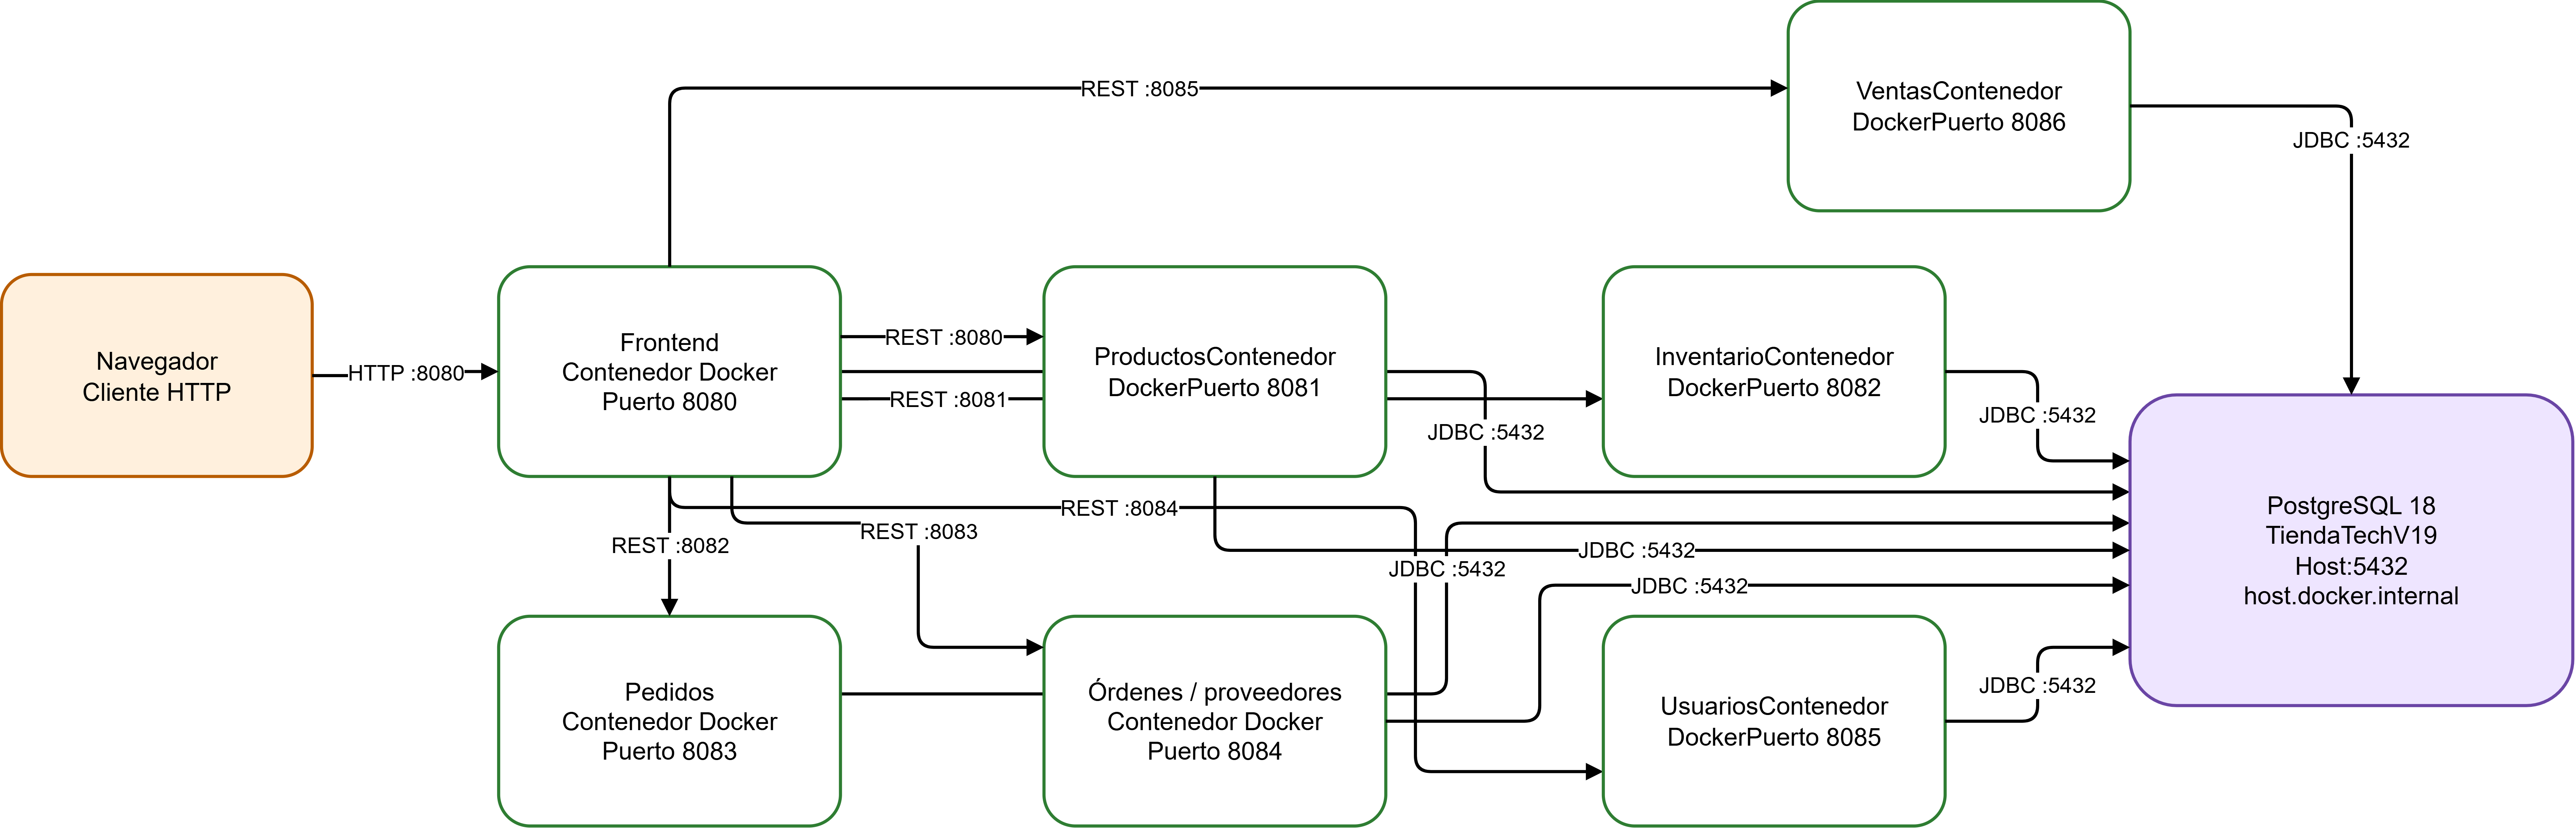
\includegraphics[width=\textwidth]{../diagrams/tiendatech-despliegue.drawio.png}
        \caption{Despliegue validado de TiendaTech mediante Docker Compose.}
        \label{fig:despliegue-e3}
    \end{figure}

    \paragraph{Comandos de despliegue}

    Para levantar todo el sistema:

    \begin{lstlisting}[style=codigo]
docker-compose up --build
    \end{lstlisting}

    Para detener y eliminar contenedores:

    \begin{lstlisting}[style=codigo]
docker-compose down
    \end{lstlisting}

    Para detener conservando los volúmenes, es decir, los datos de la base de datos:

    \begin{lstlisting}[style=codigo]
docker-compose stop
    \end{lstlisting}

    \paragraph{Dockerfile}

    \begin{lstlisting}[style=codigo,language=Dockerfile]
# syntax=docker/dockerfile:1
# ------------------------------------------
# Etapa 1: Build - compila el proyecto Java
# ------------------------------------------
FROM maven:3.9.9-eclipse-temurin-17 AS build
WORKDIR /workspace

# Forzar codificacion UTF-8 (necesario para espanol)
ENV LANG=C.UTF-8
ENV LC_ALL=C.UTF-8

# Cachea dependencias antes de copiar el codigo
COPY pom.xml .
RUN mvn -q -DskipTests dependency:go-offline

# Copia el codigo fuente y compila
COPY src ./src
RUN mvn -DskipTests clean package

# ------------------------------------------
# Etapa 2: Runtime - imagen ligera para correr
# ------------------------------------------
FROM eclipse-temurin:17-jre
WORKDIR /app

# Copia solo el JAR generado en la etapa anterior
COPY --from=build /workspace/target/*-SNAPSHOT.jar app.jar
ENV JAVA_OPTS=""

# Expone el puerto del microservicio (se sobreescribe por variable)
EXPOSE 8080
CMD ["sh", "-c", "java $JAVA_OPTS -Dserver.port=${PORT:-8080} -jar app.jar"]
    \end{lstlisting}

    \paragraph{Docker Compose}

    \begin{lstlisting}[style=codigo,language=yaml]
# ============================================================
# TiendaTech - Docker Compose
# Levanta los 6 microservicios + 6 bases de datos PostgreSQL
# Uso: docker-compose up --build
# ============================================================
services:
  # -----------------------------------------
  # MICROSERVICIO: Usuarios y Seguridad
  # Puerto: 8081 | Java / Spring Boot
  # -----------------------------------------
  usuarios-service:
    build:
      context: ./usuarios-service
      dockerfile: Dockerfile.java
    container_name: tiendatech_usuarios
    restart: always
    ports:
      - "8081:8081"
    environment:
      PORT: 8081
      SPRING_DATASOURCE_URL: jdbc:postgresql://db_usuarios:5432/db_usuarios
      SPRING_DATASOURCE_USERNAME: postgres
      SPRING_DATASOURCE_PASSWORD: 12345
      JWT_SECRET: tiendatech_jwt_secret_key
    depends_on:
      - db_usuarios
    networks:
      - tiendatech_net

  db_usuarios:
    image: postgres:17
    container_name: tiendatech_db_usuarios
    restart: always
    environment:
      POSTGRES_DB: db_usuarios
      POSTGRES_USER: postgres
      POSTGRES_PASSWORD: 12345
    ports:
      - "5433:5432"
    volumes:
      - vol_db_usuarios:/var/lib/postgresql/data
    networks:
      - tiendatech_net

  # -----------------------------------------
  # MICROSERVICIO: Productos
  # Puerto: 8082 | Python / FastAPI
  # -----------------------------------------
  productos-service:
    build:
      context: ./productos-service
      dockerfile: Dockerfile.java
    container_name: tiendatech_productos
    restart: always
    ports:
      - "8082:8082"
    environment:
      PORT: 8082
      SPRING_DATASOURCE_URL: jdbc:postgresql://db_productos:5432/db_productos
      SPRING_DATASOURCE_USERNAME: postgres
      SPRING_DATASOURCE_PASSWORD: 12345
    depends_on:
      - db_productos
    networks:
      - tiendatech_net

  db_productos:
    image: postgres:17
    container_name: tiendatech_db_productos
    restart: always
    environment:
      POSTGRES_DB: db_productos
      POSTGRES_USER: postgres
      POSTGRES_PASSWORD: 12345
    ports:
      - "5434:5432"
    volumes:
      - vol_db_productos:/var/lib/postgresql/data
    networks:
      - tiendatech_net

  # -----------------------------------------
  # MICROSERVICIO: Inventario
  # Puerto: 8083 | Java / Spring Boot
  # -----------------------------------------
  inventario-service:
    build:
      context: ./inventario-service
      dockerfile: Dockerfile.java
    container_name: tiendatech_inventario
    restart: always
    ports:
      - "8083:8083"
    environment:
      PORT: 8083
      SPRING_DATASOURCE_URL: jdbc:postgresql://db_inventario:5432/db_inventario
      SPRING_DATASOURCE_USERNAME: postgres
      SPRING_DATASOURCE_PASSWORD: 12345
      PRODUCTOS_SERVICE_URL: http://productos-service:8082
    depends_on:
      - db_inventario
      - productos-service
    networks:
      - tiendatech_net

  db_inventario:
    image: postgres:17
    container_name: tiendatech_db_inventario
    restart: always
    environment:
      POSTGRES_DB: db_inventario
      POSTGRES_USER: postgres
      POSTGRES_PASSWORD: 12345
    ports:
      - "5435:5432"
    volumes:
      - vol_db_inventario:/var/lib/postgresql/data
    networks:
      - tiendatech_net

  # -----------------------------------------
  # MICROSERVICIO: Pedidos
  # Puerto: 8084 | Java / Spring Boot
  # -----------------------------------------
  pedidos-service:
    build:
      context: ./pedidos-service
      dockerfile: Dockerfile.java
    container_name: tiendatech_pedidos
    restart: always
    ports:
      - "8084:8084"
    environment:
      PORT: 8084
      SPRING_DATASOURCE_URL: jdbc:postgresql://db_pedidos:5432/db_pedidos
      SPRING_DATASOURCE_USERNAME: postgres
      SPRING_DATASOURCE_PASSWORD: 12345
      USUARIOS_SERVICE_URL: http://usuarios-service:8081
      PRODUCTOS_SERVICE_URL: http://productos-service:8082
      INVENTARIO_SERVICE_URL: http://inventario-service:8083
    depends_on:
      - db_pedidos
      - usuarios-service
      - productos-service
      - inventario-service
    networks:
      - tiendatech_net

  db_pedidos:
    image: postgres:17
    container_name: tiendatech_db_pedidos
    restart: always
    environment:
      POSTGRES_DB: db_pedidos
      POSTGRES_USER: postgres
      POSTGRES_PASSWORD: 12345
    ports:
      - "5436:5432"
    volumes:
      - vol_db_pedidos:/var/lib/postgresql/data
    networks:
      - tiendatech_net

  # -----------------------------------------
  # MICROSERVICIO: Ventas
  # Puerto: 8085 | Java / Spring Boot
  # -----------------------------------------
  ventas-service:
    build:
      context: ./ventas-service
      dockerfile: Dockerfile.java
    container_name: tiendatech_ventas
    restart: always
    ports:
      - "8085:8085"
    environment:
      PORT: 8085
      SPRING_DATASOURCE_URL: jdbc:postgresql://db_ventas:5432/db_ventas
      SPRING_DATASOURCE_USERNAME: postgres
      SPRING_DATASOURCE_PASSWORD: 12345
      PEDIDOS_SERVICE_URL: http://pedidos-service:8084
      USUARIOS_SERVICE_URL: http://usuarios-service:8081
      INVENTARIO_SERVICE_URL: http://inventario-service:8083
      PAYPAL_CLIENT_ID: ${PAYPAL_CLIENT_ID}
      PAYPAL_CLIENT_SECRET: ${PAYPAL_CLIENT_SECRET}
    depends_on:
      - db_ventas
      - pedidos-service
      - usuarios-service
      - inventario-service
    networks:
      - tiendatech_net

  db_ventas:
    image: postgres:17
    container_name: tiendatech_db_ventas
    restart: always
    environment:
      POSTGRES_DB: db_ventas
      POSTGRES_USER: postgres
      POSTGRES_PASSWORD: 12345
    ports:
      - "5437:5432"
    volumes:
      - vol_db_ventas:/var/lib/postgresql/data
    networks:
      - tiendatech_net

  # -----------------------------------------
  # MICROSERVICIO: Ordenes y Proveedores
  # Puerto: 8086 | Java / Spring Boot
  # -----------------------------------------
  ordenes-service:
    build:
      context: ./ordenes-service
      dockerfile: Dockerfile.java
    container_name: tiendatech_ordenes
    restart: always
    ports:
      - "8086:8086"
    environment:
      PORT: 8086
      SPRING_DATASOURCE_URL: jdbc:postgresql://db_ordenes:5432/db_ordenes
      SPRING_DATASOURCE_USERNAME: postgres
      SPRING_DATASOURCE_PASSWORD: 12345
      USUARIOS_SERVICE_URL: http://usuarios-service:8081
      PRODUCTOS_SERVICE_URL: http://productos-service:8082
      INVENTARIO_SERVICE_URL: http://inventario-service:8083
    depends_on:
      - db_ordenes
      - usuarios-service
      - productos-service
      - inventario-service
    networks:
      - tiendatech_net

  db_ordenes:
    image: postgres:17
    container_name: tiendatech_db_ordenes
    restart: always
    environment:
      POSTGRES_DB: db_ordenes
      POSTGRES_USER: postgres
      POSTGRES_PASSWORD: 12345
    ports:
      - "5438:5432"
    volumes:
      - vol_db_ordenes:/var/lib/postgresql/data
    networks:
      - tiendatech_net

# -----------------------------------------
# RED: todos los servicios se comunican
# por nombre de contenedor dentro de esta red
# -----------------------------------------
networks:
  tiendatech_net:
    driver: bridge

# -----------------------------------------
# VOLUMENES: persistencia de datos de cada BD
# -----------------------------------------
volumes:
  vol_db_usuarios:
  vol_db_productos:
  vol_db_inventario:
  vol_db_pedidos:
  vol_db_ventas:
  vol_db_ordenes:
    \end{lstlisting}


    \section{Trabajos relacionados}

    El desarrollo de plataformas modernas de comercio electrónico optimizadas para la configuración de productos complejos ha impulsado una notable evolución en la literatura científica. A continuación, se presenta una síntesis integradora de los enfoques metodológicos actuales, estructurada mediante el mapeo de problemas y tecnologías de vanguardia indexadas entre los años 2020 y 2025.

    \subsection{Mapeo de Problemas y Enfoques Metodológicos}

    El primer núcleo problemático identificado en la literatura corresponde a la rigidez y la falta de contextualización en las recomendaciones tradicionales de catálogo. Trabajos como el de \textcite{vinayababu2025revolutionizing} y \textcite{khadka2025review} abordan la transición desde el filtrado colaborativo clásico hacia arquitecturas híbridas distribuidas, demostrando que la diversificación y la escalabilidad del catálogo son críticas para mitigar la sobrecarga de información en entornos transaccionales de alta concurrencia. En este sentido, la optimización matemática de estos catálogos ha sido evaluada empíricamente por \textcite{tokala2025empirical}, quien demuestra que variantes avanzadas de factorización de matrices (como SVD++) minimizan el error cuadrático medio (RMSE) en el backend analítico de las plataformas comerciales.

    El segundo desafío crítico radica en la resolución de colisiones lógicas durante la personalización adaptativa de productos. El enfoque metodológico de \textcite{velten2025solutions} introduce la programación por restricciones (Constraint Programming) como una solución óptima para modelar tablas de restricciones de ingeniería informando en tiempo real al usuario sobre conflictos mínimos y sus respectivas resoluciones. Para complementar este dinamismo sin degradar la experiencia de usuario, \textcite{benncir2025new} proponen modelos de \textit{co-clustering} explicable que no solo agrupan las preferencias multidimensionales de los clientes, sino que dotan al sistema de interpretabilidad, explicando de forma transparente la razón técnica de una sugerencia o restricción.

    Finalmente, la brecha de interacción interactiva se ha visto revolucionada por el procesamiento de lenguaje natural. \textcite{chihab2025ai} demuestran la viabilidad de clasificar automáticamente perfiles de usuarios a partir de texto no estructurado para dirigir recomendaciones basadas en competencias o necesidades explícitas. Asimismo, \textcite{munson2025review} y \textcite{sabiri2025hybrid} exponen la cúspide actual de esta evolución: la hibridación de Modelos de Lenguaje Grandes (LLMs) con sistemas de recomendación tradicionales, transitando de estructuras rígidas basadas en matrices hacia sistemas cognitivos capaces de mantener diálogos fluidos utilizando arquitecturas Transformer y recuperación aumentada de datos (RAG).

    \subsection{Tabla Comparativa de Trabajos Relacionados}

    Para sintetizar los enfoques metodológicos y contrastar el estado actual de la tecnología, la Tabla \ref{tab:estado_arte} condensa las contribuciones, ventajas y limitaciones de las fuentes indexadas seleccionadas.

    \begin{table}[htbp]
        \centering
        \caption{Matriz comparativa del Estado del Arte.}
        \label{tab:estado_arte}
        \resizebox{\textwidth}{!}{%
            \begin{tabular}{llll}
                \toprule
                \textbf{Referencia Indexada} & \textbf{Enfoque Metodológico / Tecnología} & \textbf{Ventajas Principales} & \textbf{Limitaciones Detectadas} \\ \midrule
                \textcite{vinayababu2025revolutionizing} & Encuesta de Sistemas Híbridos & Mapeo global de arquitecturas modernas. & No profundiza en validaciones lógicas de ingeniería. \\
                \textcite{sabiri2025hybrid} & Sistemas basados en Calidad y Microservicios & Alta disponibilidad y métricas de rendimiento. & Complejidad elevada en el acoplamiento de datos. \\
                \textcite{chihab2025ai} & NLP y Clasificación Supervisada & Clasificación precisa de perfiles (96.38\%). & Requiere datos pre-etiquetados masivos. \\
                \textcite{benncir2025new} & Overlapping Co-Clustering (OCCMM) & Alta interpretabilidad y explicabilidad del sistema. & Elevado consumo computacional en matrices densas. \\
                \textcite{tokala2025empirical} & Factorización de Matrices (SVD/SVD++) & Optimización matemática predictiva del catálogo. & Es un proceso estático, no apto para flujos síncronos. \\
                \textcite{velten2025solutions} & Programación por Restricciones (CP-Solver) & Resolución de conflictos mínimos en tiempo real. & Limitado a configuraciones industriales rígidas. \\
                \textcite{munson2025review} & Modelos de Lenguaje Grande (LLMs) & Interacción conversacional altamente contextual. & Riesgo latente de alucinación de datos técnicos. \\ \bottomrule
            \end{tabular}%
        }
    \end{table}

    \subsection{Declaración del Vacío Científico (Gap Statement)}

    A pesar de los avances evidenciados en el mapeo previo, la revisión de la literatura expone una desconexión metodológica entre los entornos de asistencia conversacional basados en LLM y los motores de validación por restricciones lógicas. Mientras algunas investigaciones resuelven el procesamiento conversacional de forma aislada \cite{munson2025review}, otras abordan las colisiones de componentes mediante modelos matemáticos confinados a dominios especializados \cite{velten2025solutions}. TiendaTech plantea como evolución futura la integración de ambos enfoques. La Entrega 3 no implementa esta contribución completa: proporciona y valida la infraestructura distribuida transaccional sobre la cual podría incorporarse posteriormente.

    \subsection{Distribución de datos: fragmentación y colocalización}

    El eje revisado en las subsecciones anteriores corresponde al problema heredado de E1 y E2, centrado en la recomendación y la validación de compatibilidad. La Entrega 3 incorpora un segundo eje, propio de esta etapa: la distribución del dominio transaccional y el procesamiento analítico sobre el historial de pedidos. Concretamente, el esquema implementado fragmenta \texttt{pedidos.orden} por trimestres de \texttt{fecha} y favorece el acceso conjunto de \texttt{usuarios.usuario} $\ltimes$ \texttt{pedidos.orden} mediante \texttt{usuario\_id}. Sobre ese historial, el avance ejecuta un análisis top-N trimestral y una segmentación monetaria de clientes; el recomendador colaborativo y la segmentación RFM completa permanecen como extensiones posteriores. Las subsecciones siguientes revisan la literatura indexada del período 2020--2024 para esos frentes.

    \textcite{ozsu2020} establecen el marco con el que se justifica el esquema adoptado: la distinción entre fragmentación horizontal primaria, definida por predicados sobre la propia relación, y derivada, que propaga el predicado mediante la semi-unión, junto con las reglas de corrección que todo particionamiento debe satisfacer. Su tratamiento es analítico y supone conocida la carga de consultas. \textcite{liu2024} recorren el estado del arte del particionamiento de datos y muestran que las propuestas actuales se organizan según el entorno de despliegue y se apoyan en características del esquema, de los datos, de la carga y de métricas de ejecución, con etapas diferenciadas de inicialización y optimización del esquema. \textcite{abdalla2023} avanzan en esa dirección mediante un enfoque basado en agrupamiento jerárquico para el diseño de bases relacionales distribuidas.

    Ambos trabajos recientes apuntan a la generación automática del esquema sobre cargas sintéticas. Ninguno aborda el caso inverso, que es el de este avance: un esquema derivado manualmente desde un conjunto pequeño y fijo de consultas de negocio, cuya validación consiste en comprobar que esas consultas efectivamente descartan particiones al ejecutarse.

    Dos propuestas recientes muestran hasta dónde ha llegado esa automatización. \textcite{kang2021jigsaw} plantean un motor de almacenamiento con particiones irregulares guiadas por la carga, orientado a reducir la lectura de datos no solicitados, y \textcite{zhou2023grep} seleccionan las claves de particionado mediante aprendizaje sobre grafos. Ambas suponen la disponibilidad de trazas de ejecución suficientes para alimentar la decisión, condición que no se cumple en un sistema que todavía no ha entrado en operación. Por esa razón el esquema de este avance se deriva de las consultas de referencia declaradas y no de un histórico observado.

    \subsection{Motores SQL distribuidos}

    \textcite{taft2020} describen un motor que fragmenta las tablas en rangos ordenados por clave, los replica por consenso y designa un \emph{leaseholder} por rango, mientras la capa SQL empuja los operadores hacia los nodos que poseen los datos. El trabajo reporta que los rangos se dividen tanto por tamaño como por carga para reducir puntos calientes, y evalúa el sistema sobre cargas OLTP de tipo industrial y despliegues multirregión.

    Dos aspectos quedan fuera de ese alcance y son los que importan para este avance. Primero, no se examina un esquema particionado por fecha, donde las escrituras se concentran por construcción en el rango más reciente; la división por carga mitiga el desbalance, pero el análisis no cubre ese patrón. Segundo, la evaluación se realiza sobre clústeres de decenas de nodos, de modo que el comportamiento en un despliegue reducido no se deriva de esos resultados y debe medirse de forma independiente.

    En el plano de la verificación, \textcite{rigger2020querypartitioning} muestran que descomponer una consulta en particiones lógicas equivalentes y comparar sus resultados permite detectar errores de correctitud en gestores relacionales, incluido CockroachDB. La técnica pertenece a la prueba de software y no al diseño físico de la distribución, pero resulta pertinente aquí porque advierte que un motor distribuido puede devolver resultados incorrectos sin fallar de forma visible, un riesgo que ninguna medición de latencia detecta.

    \subsection{Analítica paralela sobre el historial transaccional}

    \textcite{ahmed2020} comparan el desempeño de Hadoop y Spark sobre conjuntos de datos de gran escala con la suite HiBench, y fijan el tipo de evidencia experimental que se espera de esta clase de medición: cargas diversas, tamaños crecientes y repeticiones por configuración. El régimen que estudian, sin embargo, es el opuesto al de este avance: allí el cómputo útil domina el tiempo total, mientras que en un historial de pedidos de escala académica el costo fijo de coordinación pesa proporcionalmente mucho más. Esa diferencia no es un detalle de magnitud, sino la condición que determina si el procesamiento se acelera o se degrada al añadir recursos.

    \subsection{Límites del paralelismo}

    \textcite{ahmed2021} constituyen el antecedente más directo para la medición del procesamiento paralelo. Sobre un clúster físico de un nodo maestro y nueve esclavos, muestran que en varias cargas de Spark el tiempo de ejecución \emph{aumenta} al agregar ejecutores, porque la porción serial crece de forma proporcional a la raíz del número de ejecutores. A partir de esa observación proponen el modelo

    \begin{equation}
        t = \frac{a}{n_{ejec}} + b\sqrt{n_{ejec}}
        \label{eq:modelo-paralelizacion}
    \end{equation}

    donde $t$ es el tiempo de ejecución, $n_{ejec}$ el número de ejecutores, y $a$ y $b$ constantes ajustadas empíricamente para un tamaño de problema fijo.

    Al contrastar el ajuste del modelo con las dos cotas clásicas mediante el coeficiente de determinación, la Ecuación \eqref{eq:modelo-paralelizacion} resulta mejor en 25 de 35 curvas, frente a 4 de la formulación de Amdahl \cite{amdahl1967} y 6 de la de Gustafson \cite{gustafson1988}. Dos consecuencias son aplicables a la definición de las métricas de esta entrega. La primera es que las cotas clásicas describen únicamente el caso en que el tiempo desciende hasta converger, y no el caso en que se degrada. La segunda es que con tamaños de problema pequeños los costos generales del clúster llegan a opacar el patrón, lo que obliga a reportar el volumen procesado junto a cualquier medición de aceleración. Por ambas razones, las cotas de Amdahl y Gustafson se adoptan como referencia de contraste del \emph{speedup} observado y no como valor esperado.

    \subsection{Matriz comparativa del eje de distribución y analítica}

    De forma análoga a la Tabla \ref{tab:estado_arte}, la Tabla \ref{tab:estado_arte_distribucion} condensa el aporte de cada fuente de este segundo eje y la limitación que deja abierta respecto del alcance de la Entrega 3.

    \begin{table}[htbp]
        \centering
        \caption{Matriz comparativa del eje de distribución de datos y analítica paralela.}
        \label{tab:estado_arte_distribucion}
        \small
        \begin{tabularx}{\textwidth}{p{3cm} X X}
\toprule
\textbf{Referencia} & \textbf{Aporte principal} & \textbf{Limitación para este avance} \\
\midrule
\textcite{ozsu2020} & Marco formal de fragmentación primaria y derivada. & Supone conocida la carga de consultas. \\
\textcite{taft2020} & Rangos ordenados, consenso y capa SQL distribuida. & Clústeres de decenas de nodos; sin particionamiento por fecha. \\
\textcite{ahmed2020} & Comparativa Hadoop--Spark con la suite HiBench. & Volúmenes en los que el cómputo útil domina. \\
\textcite{rigger2020querypartitioning} & Detección de errores lógicos por partición de consultas. & Técnica de prueba, no de diseño físico. \\
\textcite{kang2021jigsaw} & Particiones irregulares guiadas por la carga. & Requiere trazas de ejecución previas. \\
\textcite{ahmed2021} & Modelo de paralelización contrastado contra las cotas clásicas. & Ajustado a cargas HiBench, no de comercio electrónico. \\
\textcite{zhou2023grep} & Selección de claves mediante aprendizaje sobre grafos. & Requiere histórico de ejecución. \\
\textcite{abdalla2023} & Diseño de bases distribuidas por agrupamiento jerárquico. & Validado sobre cargas sintéticas. \\
\textcite{liu2024} & Revisión del estado del arte del particionamiento. & Orientada a la generación automática del esquema. \\
\bottomrule
        \end{tabularx}
    \end{table}

    \subsection{Posición del avance E3 en este eje}

    Los trabajos revisados abordan las piezas por separado y a escalas mayores: el diseño del particionamiento como problema de optimización automática alimentado por trazas de ejecución, el motor distribuido como sistema evaluado en clústeres grandes, y el desempeño del procesamiento paralelo en volúmenes donde la coordinación resulta despreciable. La aportación propia de esta etapa consiste en derivar el esquema de fragmentación y colocalización a partir de un conjunto acotado de consultas de negocio declaradas de antemano, y en medir la aceleración observada en el régimen de datos donde, según la literatura reciente, las cotas teóricas dejan de ser confiables.

    \subsubsection*{Nota sobre las fuentes primarias}

    Las referencias \cite{amdahl1967}, \cite{gustafson1988} y \cite{zhou2008} corresponden a formulaciones anteriores al período de revisión y se conservan porque la atribución de un método exige citar su fuente original: las dos cotas clásicas de aceleración y el algoritmo de mínimos cuadrados alternados sobre el que se construyen los recomendadores colaborativos distribuidos. La discusión del estado del arte de este eje se apoya en las nueve fuentes indexadas del período 2020--2024 recogidas en la Tabla \ref{tab:estado_arte_distribucion}.

    \section{Decisiones arquitectónicas y criterios de calidad heredados}

    \subsection{Registros de decisiones arquitectónicas ADR}

    \subsubsection{ADR-01: Arquitectura basada en microservicios}

    \textbf{Estado:} Aceptado.

    \textbf{Alternativas consideradas:} Arquitectura monolítica, descartada por el alto acoplamiento entre módulos; y arquitectura en capas N-tier, descartada por sus limitaciones para escalar servicios de forma independiente.

    \textbf{Decisión:} Se adopta una arquitectura basada en microservicios para usuarios, productos, inventario, pedidos, órdenes a proveedores y ventas. El frontend centraliza el acceso y el enrutamiento hacia estos servicios.

    \textbf{Justificación:} Esta arquitectura permite separar responsabilidades, escalar módulos específicos y reducir el impacto de fallos. Por ejemplo, un problema en el catálogo no debería afectar directamente el procesamiento de pagos.

    \textbf{Consecuencia:} Mejora la escalabilidad, disponibilidad y mantenibilidad del sistema, aunque incrementa la complejidad de comunicación entre servicios.

    \subsubsection{ADR-02: Enrutamiento centralizado en el frontend}

    \textbf{Estado:} Aceptado.

    \textbf{Alternativas consideradas:} Comunicación directa entre cliente y microservicios, descartada por riesgos de seguridad y mayor acoplamiento; y Backend for Frontend, descartado porque en esta fase solo se contempla un cliente web principal.

    \textbf{Decisión:} El componente frontend incorpora Spring Cloud Gateway y funciona como punto de entrada para las solicitudes del cliente web.

    \textbf{Justificación:} El enrutamiento centralizado evita que el cliente necesite conocer las direcciones internas de cada servicio y concentra la configuración de rutas. La autenticación permanece principalmente en el servicio de usuarios, por lo que no se atribuyen al gateway controles que todavía no han sido verificados.

    \textbf{Consecuencia:} Facilita el control de solicitudes y la organización de la arquitectura, pero se convierte en un componente crítico que debe manejarse con tolerancia a fallos.

    \subsubsection{ADR-03: Motor de compatibilidad como microservicio independiente}

    \textbf{Estado:} Propuesto; no implementado en la Entrega 3.

    \textbf{Alternativas consideradas:} Incluir la lógica de compatibilidad dentro del catálogo, descartado por mezclar responsabilidades; y validar la compatibilidad en el frontend, descartado por riesgos de manipulación y baja confiabilidad.

    \textbf{Decisión:} Se propone implementar el motor de compatibilidad de hardware como un microservicio especializado en una entrega posterior.

    \textbf{Justificación:} La validación entre procesador, placa madre, RAM, GPU, almacenamiento y fuente de poder requiere reglas técnicas que pueden cambiar con frecuencia. Separar este módulo permite actualizar las reglas sin modificar el catálogo, el carrito o los pagos.

    \textbf{Consecuencia:} Mejora la precisión y mantenibilidad del sistema, aunque requiere comunicación constante con el catálogo de productos para mantener actualizada la información técnica.

    \subsection{Métricas de calidad basadas en ISO/IEC 25010}

    Las métricas se definen para evaluar atributos de calidad relevantes en \textbf{TiendaTech}, especialmente rendimiento, disponibilidad, fiabilidad, seguridad, mantenibilidad y compatibilidad funcional.

    \begin{table}[htbp]
        \centering
        \caption{Métricas de calidad basadas en ISO/IEC 25010 para TiendaTech.}
        \label{tab:metricas_iso25010}
        \resizebox{\textwidth}{!}{%
            \begin{tabular}{llll}
                \toprule
                \textbf{Característica} & \textbf{Métrica conocida} & \textbf{Forma de medición / fórmula} & \textbf{Umbral objetivo} \\
                \midrule
                Rendimiento & Tiempo de respuesta P95 &
                Ordenar los tiempos de respuesta y tomar el valor donde se ubica el 95\% de solicitudes. &
                $\leq 500$ ms \\

                Rendimiento & Throughput &
                $\frac{\text{Total de solicitudes procesadas}}{\text{Tiempo total de prueba}}$ &
                $\geq 30$ req/s \\

                Disponibilidad & Uptime &
                $\frac{\text{Tiempo activo del sistema}}{\text{Tiempo total de operación}} \times 100$ &
                $\geq 99\%$ \\

                Fiabilidad & Error Rate &
                $\frac{\text{Solicitudes fallidas}}{\text{Total de solicitudes}} \times 100$ &
                $\leq 1\%$ \\

                Mantenibilidad & MTTR &
                $\frac{\text{Tiempo total de reparación}}{\text{Número de incidentes corregidos}}$ &
                $\leq 2$ horas \\

                Seguridad & Tasa de bloqueo de accesos no autorizados &
                $\frac{\text{Intentos no autorizados bloqueados}}{\text{Total de intentos no autorizados}} \times 100$ &
                $\geq 99\%$ \\

                Compatibilidad funcional &
                Tasa de pruebas funcionales aprobadas &
                $\frac{\text{Casos de prueba aprobados}}{\text{Total de casos de prueba ejecutados}} \times 100$ &
                $\geq 95\%$ \\
                \bottomrule
            \end{tabular}%
        }
    \end{table}

    Estas métricas cubren los aspectos más importantes de \textbf{TiendaTech}. En esta fase se priorizan el rendimiento, la disponibilidad, la fiabilidad, la seguridad y la compatibilidad funcional, porque afectan directamente la experiencia del usuario y la correcta validación de los componentes de hardware.


    \newpage

    \section{Registro de Cambios respecto a la Entrega 2}

    La tercera entrega transforma el diseño arquitectónico de la Entrega 2 en una implementación distribuida verificable. Los cambios incorporados cubren construcción, despliegue, integración entre servicios, persistencia y validación cuantitativa. La Tabla
    \ref{tab:registro_cambios} resume los cambios más relevantes.

    \begin{table}[H]
        \centering
        \caption{Registro de cambios respecto a la Entrega 2}
        \label{tab:registro_cambios}
        \small
        \begin{tabularx}{\textwidth}{p{2.8cm} p{2.8cm} p{3.2cm} X}
\toprule
\textbf{Aspecto} & \textbf{Entrega 2} & \textbf{Entrega 3} & \textbf{Evidencia verificable} \\
\midrule

Arquitectura &
Microservicios definidos conceptualmente &
Frontend y seis microservicios implementados &
Siete imágenes Docker construidas y siete contenedores activos. \\
\midrule

Comunicación &
Contratos REST propuestos &
Clientes REST integrados entre dominios &
Pedidos consulta usuarios y productos, genera facturas y activa movimientos de inventario. \\
\midrule

Despliegue &
Estrategia Docker documentada &
Docker Compose ejecutable &
Puertos 8080--8086 y conexión a PostgreSQL mediante \texttt{host.docker.internal}. \\
\midrule

Persistencia &
Modelo y rutinas iniciales &
Esquemas y migraciones alineados con V19 &
Facturación vinculada con órdenes particionadas y kardex compatible con entradas y salidas. \\
\midrule

Validación funcional &
Sin ejecución integral documentada &
Flujo transaccional completo &
Orden 19, factura \texttt{FAC-000006} y reducción de stock de 240 a 239. \\
\midrule

Rendimiento &
Métricas objetivo definidas &
Métricas observadas &
210 solicitudes, 100\,\% de éxito y P95 máximo de 51,94~ms. \\
\midrule

Alcance &
Servicios futuros incluidos en el diseño &
Estado real diferenciado del alcance futuro &
El motor de compatibilidad y otras capacidades no implementadas se mantienen como trabajo posterior. \\

\bottomrule
        \end{tabularx}
    \end{table}

    Estos cambios permiten que la propuesta evolucione desde una arquitectura documentada hacia un sistema distribuido ejecutable. La evidencia de esta entrega se limita a las capacidades comprobadas en el repositorio y distingue explícitamente los componentes implementados de aquellos que permanecen como trabajo futuro.

    \newpage

    \section{Resultados de la Entrega 3}

    \subsection{Entorno verificado}

    La validación se realizó en un entorno local con Docker Compose y PostgreSQL 18. La base de datos utilizada fue \texttt{TiendaTechV19}, accesible desde los contenedores mediante \path{host.docker.internal}. El despliegue estuvo compuesto por un frontend en el puerto 8080 y seis servicios backend en los puertos 8081 a 8086. La Tabla \ref{tab:componentes_e3} resume el inventario comprobado.

    \begin{table}[H]
        \centering
        \caption{Componentes desplegados y verificados en la Entrega 3}
        \label{tab:componentes_e3}
        \small
        \begin{tabularx}{\textwidth}{X c X c}
\toprule
\textbf{Componente} & \textbf{Puerto} & \textbf{Responsabilidad} & \textbf{Estado} \\
\midrule
Frontend & 8080 & Punto de entrada y enrutamiento & Operativo \\
Productos & 8081 & Catálogo, precio e IVA & Operativo \\
Inventario & 8082 & Stock y movimientos & Operativo \\
Pedidos & 8083 & Carrito, orden y checkout & Operativo \\
Órdenes a proveedores & 8084 & Proveedores y abastecimiento & Operativo \\
Usuarios & 8085 & Usuarios, autenticación y direcciones & Operativo \\
Ventas & 8086 & Facturación y coordinación con inventario & Operativo \\
\bottomrule
        \end{tabularx}
    \end{table}

    \subsection{Flujo transaccional comprobado}

    El caso integral validado utilizó el usuario 47, la dirección 10 y el producto 4. El servicio de pedidos obtuvo los datos de usuario y producto mediante REST, creó la orden 19 y solicitó la facturación al servicio de ventas. Como resultado se generó la factura \texttt{FAC-000006}. Posteriormente, ventas solicitó al servicio de inventario un movimiento de salida asociado a la referencia \texttt{FAC-6}, con lo cual el stock disminuyó de 240 a 239 unidades.

    \begin{table}[H]
        \centering
        \caption{Trazabilidad del flujo distribuido validado}
        \label{tab:flujo_validado}
        \small
        \begin{tabularx}{\textwidth}{p{3.2cm} X X}
\toprule
\textbf{Etapa} & \textbf{Resultado} & \textbf{Evidencia} \\
\midrule
Preparación del carrito & Producto 4, cantidad 1 & Precio unitario de 214,99 \\
Creación de orden & Orden 19 & Total de 214,99 \\
Facturación & Factura 6 & Número \texttt{FAC-000006} \\
Movimiento de inventario & Salida por venta & Movimiento 41, referencia \texttt{FAC-6} \\
Actualización de stock & Descuento de una unidad & Stock de 240 a 239 \\
\bottomrule
        \end{tabularx}
    \end{table}

    \subsection{Pruebas funcionales}

    Se ejecutaron diez casos funcionales sobre construcción, arranque, consulta de datos, checkout, facturación, inventario y búsqueda de usuarios. Los diez casos finalizaron satisfactoriamente, por lo que la tasa funcional observada fue:

    \[
        \text{Tasa de aprobación} =
        \frac{10\ \text{casos aprobados}}{10\ \text{casos ejecutados}}
        \times 100 = 100.
    \]

    Por tanto, la tasa de aprobación obtenida fue del 100\,\%.

    Esta validación demuestra la operatividad del recorrido seleccionado para E3, pero no sustituye pruebas de estrés, seguridad, recuperación ante fallos o concurrencia, que requieren escenarios y herramientas específicas.

    \subsection{Resultados de rendimiento}

    Se realizaron 30 solicitudes secuenciales de lectura sobre cada uno de los siete componentes, para un total de 210 observaciones. Todas las solicitudes obtuvieron una respuesta HTTP satisfactoria. La Tabla \ref{tab:metricas_e3} presenta los tiempos observados.

    \begin{table}[H]
        \centering
        \caption{Tiempos de respuesta observados en 30 repeticiones por componente}
        \label{tab:metricas_e3}
        \small
        \begin{tabular}{lrrrr}
            \toprule
            \textbf{Servicio} & \textbf{Éxito} & \textbf{Promedio (ms)} & \textbf{P95 (ms)} & \textbf{Máximo (ms)} \\
            \midrule
            Frontend & 100\,\% & 41,46 & 46,22 & 133,04 \\
            Productos & 100\,\% & 25,34 & 51,94 & 126,83 \\
            Inventario & 100\,\% & 11,93 & 13,24 & 18,64 \\
            Pedidos & 100\,\% & 13,21 & 19,01 & 20,81 \\
            Proveedores & 100\,\% & 13,24 & 16,67 & 17,89 \\
            Usuarios & 100\,\% & 15,22 & 21,70 & 25,77 \\
            Ventas & 100\,\% & 12,46 & 16,26 & 18,03 \\
            \bottomrule
        \end{tabular}
    \end{table}

    El mayor P95 correspondió al servicio de productos con 51,94~ms, resultado inferior al umbral de 500~ms definido en la Entrega 2. Debido a que las solicitudes fueron secuenciales y ejecutadas en un entorno local, estos valores caracterizan el escenario de validación, pero no deben interpretarse como capacidad bajo carga concurrente ni como evidencia de disponibilidad en producción.

    \subsection{Hallazgos técnicos y acciones correctivas}

    Durante la integración se identificaron incompatibilidades entre la estructura actual de la base y algunas rutinas. Se alineó el encabezado de factura con la clave compuesta de la tabla particionada de órdenes, se actualizó la restricción del kardex para aceptar los tipos usados por la rutina de movimientos y se habilitó la extensión \texttt{unaccent} requerida por la búsqueda de usuarios. Estas correcciones fueron implementadas como migraciones idempotentes y aplicadas sobre \texttt{TiendaTechV19}.

    \subsection{Limitaciones y trabajo pendiente}

    La implementación actual utiliza una base PostgreSQL compartida entre los servicios, por lo que todavía existe acoplamiento a nivel de persistencia. Asimismo, las mediciones realizadas no incorporan concurrencia, latencia de red externa ni inyección de fallos. El motor de compatibilidad de hardware y otras capacidades descritas en el diseño previo no aparecen como servicios implementados en el despliegue validado; en consecuencia, se mantienen como alcance posterior y no se presentan como resultados de esta entrega.

    \newpage




    \newpage
    \printbibliography[title={Referencias}]

\end{document}
